%!TEX root = ../Thesis.tex

\chapter{Workshop 3}
\lhead{}
Deelnemers: Danny, Huib

De workshop begon met een uitleg over de implementatie van de LookEvents uit de VRInteractions plugin en de verschillende configuratie mogelijkheden. Daarnaast is gezamenlijk een vergelijkbare functionaliteit gemaakt zodat het probleem van een node naam niet weten, uit Workshop 2, niet meer voor zou komen.

\section{Doel}
Een ingewikkelder versie van de LookEvents implementeren met hierin:

\begin{itemize}
	\item Meerdere look events in een Actor
	\item Veranderden van een material tijdens runtime
	\item Het gebruik en maken van een functie
	\item Het gebruik en maken van variabel
\end{itemize}

\section{Opdrachten}

We gaan een bank maken waar een menu boven zweeft waarmee wij het materiaal van de bank kunnen kiezen. Het menu word zichtbaar op het moment dat er naar de bank gekeken word.

\subsection{Opdracht 1}
Maak van de bank een Blueprint en voeg hier een scene (dit is een component) aan toe genaamd options met daarin drie static meshes genaamd option0 t/m option2.

Voeg voor elk element een Lookevent component toe en noem die LookEventOption0 t/m LookEventOption2.

\begin{figure}[!ht]
  \centering
    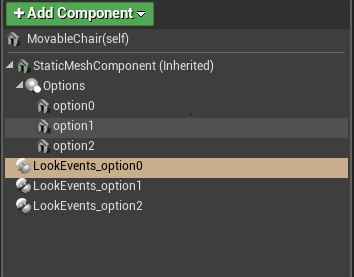
\includegraphics[width=\linewidth,height=\textheight,keepaspectratio]{Workshop_3_AddComponentExample}
    \caption{Voorbeeld van het toevoegen van de LookEvents componenten aan een Actor.}
\end{figure}

Koppel de look events aan de juiste options, kijk hiervoor naar de vorige opdracht, en zet de optie  “Draw debug trigger” aan zodat je makkelijk kan zien of alles werkt.

\subsection{Opdracht 2}
Om te zorgen dat de options alleen zichtbaar worden als er naar de bank gekeken word voegen we nog een LookEvents component toe genaamd “LookEventsMain”. 

Om de code schoner te houden maken we een functie genaamd “SetOptionsVisibility” met boolean als input genaamd “Visibility”. In deze functie haal je alle kinderen van de Options scene component op en zet je de visibility hiervan op de input.

\begin{figure}[!ht]
  \centering
    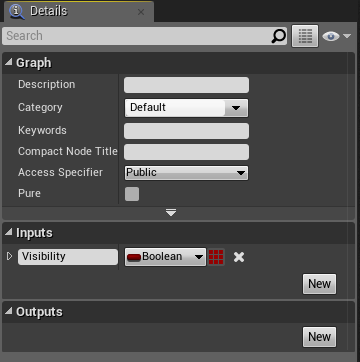
\includegraphics[width=\linewidth,height=\textheight,keepaspectratio]{Workshop_3_functieVoorbeeld}
    \caption{Voorbeeld van een functie in Blueprints.}
\end{figure}

Koppel nu de OnSeen en de OnUnseen events van de “LookEventsMain” aan de “SetOptionsVisibility” functie.

\subsection{Opdracht 3}
We gebruiken de materials van de options static meshes om de material van de bank te bepalen. Op het moment dat er naar een option gekeken word (dus het OnSeen event) halen we de material uit de bijhorende option en zetten we material van de hoofd static mesh hierop

\subsection{Opdracht 4}
Probeer niet de material maar de mesh van de bank te veranderden. Je kan dit do en via de static meshes van de options (zelfde manier als wij de kleuren maken) maar als je een uitdaging wilt probeer het via een array variable.

\begin{figure}[!ht]
  \centering
    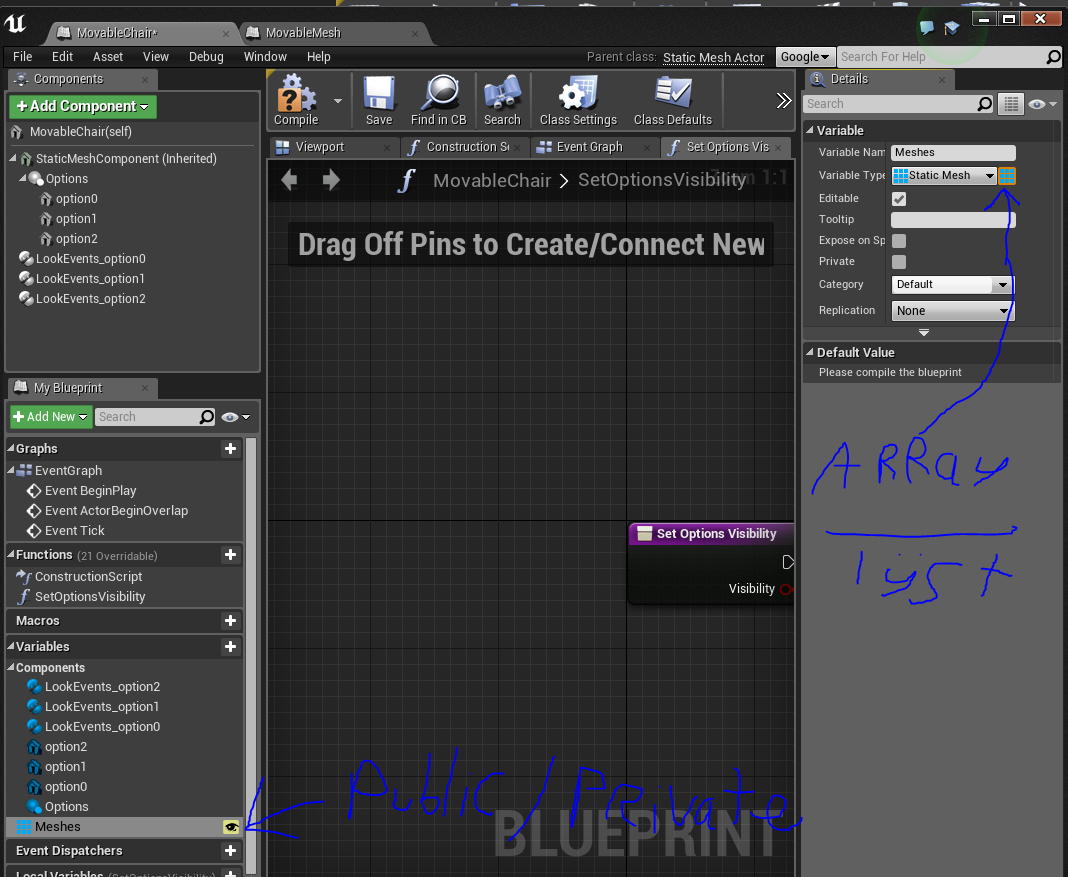
\includegraphics[width=\linewidth,height=\textheight,keepaspectratio]{Workshop_3_variableVoorbeeld}
    \caption{Voorbeeld van een variable in Blueprints.}
\end{figure}

Als je voor een variabel gaat vergeet niet dat dit een lijst van Static Mesh References moet zijn.

\section{Reflectie}
Na het bespreken van de opdracht werd er aangegeven dat er minder tijd kwijt aan het zoeken naar functie namen omdat een gelijke opdracht van te voren samen gemaakt was. 

Het viel op dat concepten waar in de vorige workshop problemen mee waren dit keer wel goed gingen, bijvoorbeeld het correct zetten van de LookEvents trigger, zonder hier specifieke instructies voor te geven.